\newcommand{\FigIdentifySender}{
\begin{figure}[t]
    \centering
    \includegraphics[width=0.9\linewidth]{figs/linegraph.png}
    \caption{\textbf{Messages needed to identify sender}\,---\,% 
        We measured the number of epochs that were necessary for an attacker to
        uniquely determine who was messaging a pre-selected victim, Bob, under
        sealed sender assuming every message was ``immediately'' replied to with
        a \textit{delivery receipt}. We found that the graph structure had no
        influence on the effectiveness of the attack. We ran the attack 100
        times for each user base size and found that with a user base of
        1,000,000 on average Bob needed to receive 6.5 message from the same
        user in order to deanonymize the conversation between the sender (Alice)
        and Bob.
        }
    \label{fig:signal-NumMessages}
\end{figure}
}

\newcommand{\MessageStages}{
\begin{figure}[t]
    \centering
    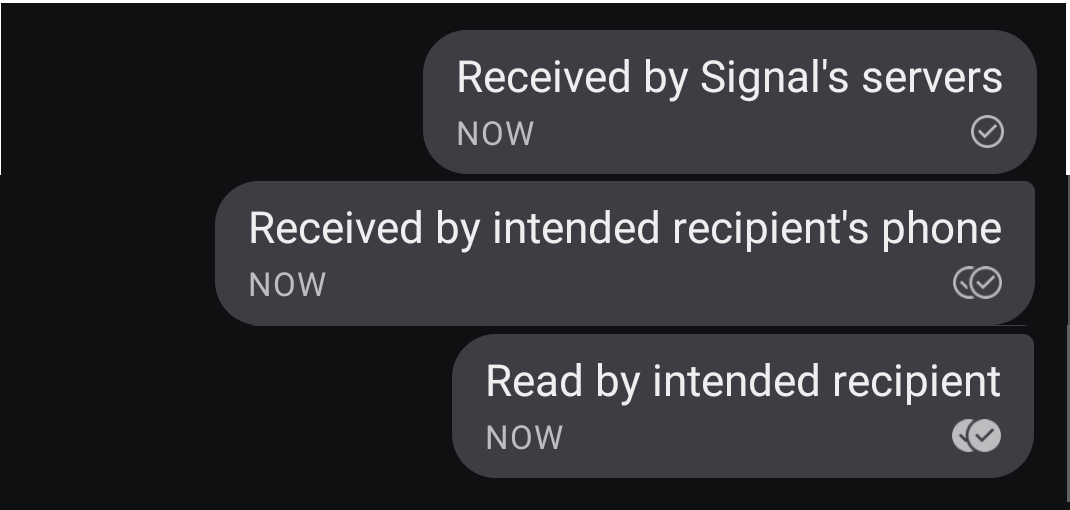
\includegraphics[width=0.8\linewidth]{figs/message-stages.png}
    \caption{\textbf{Stages of a Signal Message}\,---\,% 
        User Interface indicating message delivery status.
        % 
        One hollow check mark signifies that the message is en route. 
        %
        Two hollow check marks signifies the receipt of a delivery receipt for the message.
        %
        Finally, two filled check mark signifies the receipt of a read receipt for the message.
        %
    }
    \label{fig:signal-message-stages}
\end{figure}
}

\newcommand{\DeliveryTimeCDF}{
    \begin{figure}[t]
        \centering
        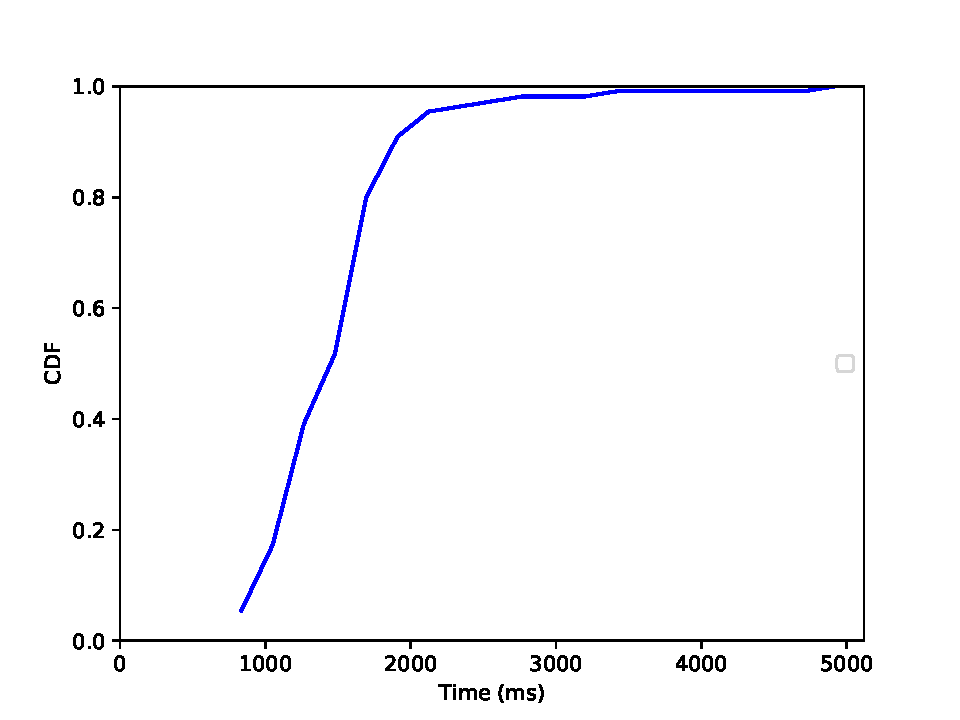
\includegraphics[width=0.8\linewidth]{figs/DRCDF.pdf}
        \caption{\textbf{CDF of Delivery Receipt timing}\,---\,%
        CDF of time between a device sending a message (to another online
        device) and receiving a Delivery Receipt. The median time is 1480ms and
        90\% of Delivery Receipts were received within 1909ms.
        }
        \label{fig:signal-delivery-cdf}
    \end{figure}
}

\newcommand{\EpochEffect}{
\begin{figure}[t]
    \centering
    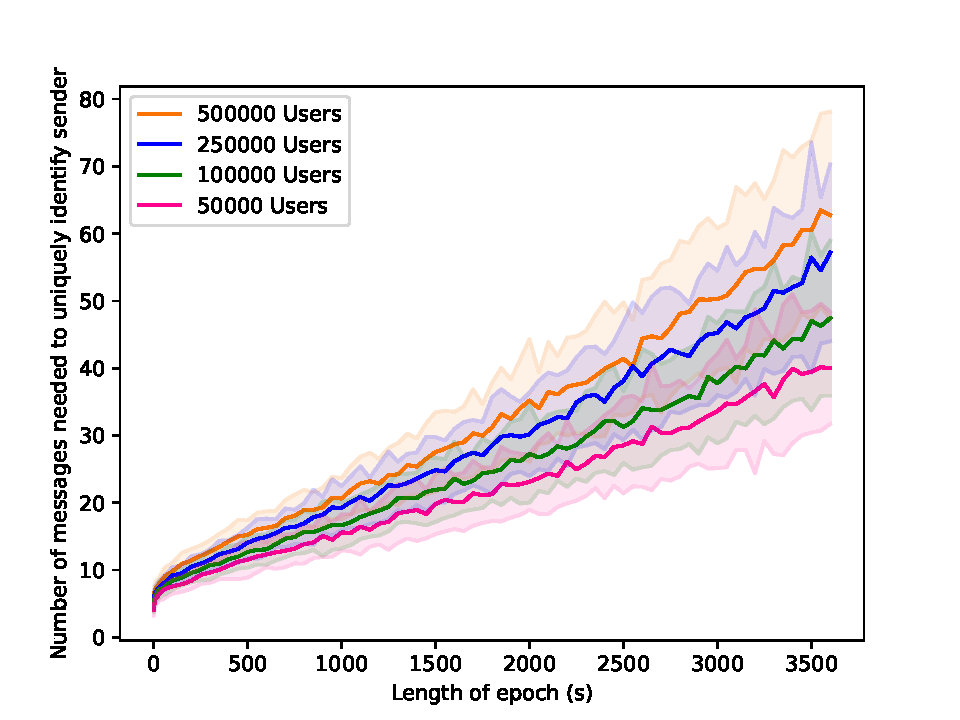
\includegraphics[width=0.9\linewidth]{figs/epoch_effect-bars.pdf}
    \caption{\textbf{Effect of delayed Read Receipts}\,---\,% 
        The attack assumes that each epoch lasts one second, and thus the log
        collects all delivery receipts that are sent within 1 second of Bob 
        receiving a sealed sender message. A possible simple solution to this
        attack is to delay (randomly per message, or publishing read receipts in
        batches) read receipts. We tested the effectiveness of the attack with
        variably sized epochs and determined that if delivery receipts were
        delayed a full hour (making them effectively worthless for their
        purpose) that with a user base of 500,000 users (each sending 50
        messages a day) Bob would need to receive 60 messages from the victim
        user to identify Alice as the sender.
        }
    \label{fig:signal-epoch-effect}
\end{figure}
}

\newcommand{\ListVsC}{
\begin{figure}[ht]
    \centering
    \includegraphics[width=0.9\linewidth]{figs/list_vs_graph.png}
    \caption{\textbf{Comparison between Python List model and Generated Graph
        Models}\,---\,% 
        After determining that the structure of the userbase graph had no effect
        on the simplified base attack (Figure~\ref{fig:NumMessages}) we modified
        our attack using Python to use a complete graph for the user base (any
        user might message any other user) and measure the effect of how
        receipts are generated for the log. In the simplified base attack the
        receipts in each epoch are structured to be 50\% random receipts, 25\%
        to be repeated receipts from a previous epoch, and 25\% receipts
        generated from replies to messages from previous epochs. As the nature
        of this attack is to only examine the `To' field of the message we
        expected only the 25\% of receipts that are repeated receipts to have
        any effect on the attack. As such we modeled our Python version to only
        have a delivery receipt from Bob to Alice and the 25\% repeated receipts
        from a previous epoch and compared to our previous models and found that
        the simplified Python model was a near match.
    }
    \label{fig:signal-listVsC}
\end{figure}
}

\newcommand{\PercentageEffect}{
\begin{figure}[t]
    \centering
    \includegraphics[width=0.9\linewidth]{figs/percentage_effect.png}
    \caption{\textbf{Effect of varying the percentage of messages in an Epoch
        that are repeated receipts}\,---\,% 
        We measured the effect of varying what percentage of an epoch's messages
        are repeated receipts from a previous epoch. As expected the larger the
        percentage, more messages persist in the recurring intersection and as
        such the attack requires more messages to identify Alice as the sender
        to Bob.
    }
    \label{fig:signal-percentageEffect}
\end{figure}
}

\newcommand{\PercentileGraph}{
\begin{figure}[ht]
    \centering
    \includegraphics[width=0.9\linewidth]{figs/Alice_percentile.pdf}
    \caption{\textbf{Alice's Percentile rank after $N$ messages}\,---\,% 
        In the full attack the number of times each user shows up in the 'To:'
        field of a Sealed Sender message in the epoch following Bob receiving a
        message is tracked. This Counter can be used to determine who is most
        likely the user in conversation with Bob. After each epoch the attacker
        can look at which users have received a message (or receipt or Typing
        Notification) most often shortly after Bob received a message. This
        graph shows Alice's precentile rank after $N$ messages---the percentage
        of users she is more likely than to be the user conversing with Bob.
    }
    \label{fig:signal-AlicePercentile}
\end{figure}
}

\newcommand{\LikelihoodGraphOld}{
\begin{figure}[ht]
    \centering
    \includegraphics[width=0.9\linewidth]{figs/Likelihood_Alice.pdf}
    \caption{\textbf{Likelihood of guessing Alice is the sender}\,---\,% 
        The natural candidate for who is messaging Bob is the user who shows up
        most often in the epoch following Bob receiving a message. This graph
        analyzes the likelihood that the attacker will be correct if they guess
        the user who has show up most often is conversing with Bob as a function
        of the number of messages Bob has received.
    }
    \label{fig:signal-AliceLikelihoodOld}
\end{figure}
}

\newcommand{\RankGraph}{
\begin{figure}[t]
    \centering
    \includegraphics[width=0.9\linewidth]{figs/Alice_rank_receipt_response_rate.pdf}
        \caption{\textbf{Number of users with Alice's count or higher after $N$ messages}\,---\,% 
        In Attack~2, we count the number of times a user receives a message in the epoch
        immediately following a message sent to Bob. This graph shows the number of users that
        have the same or higher count as Alice (the ``true'' sender in our simulation) as more
        messages are sent. We vary the percent ($f$) of epochs that send responses to Alice,
        to represent the fraction $(1-f)$ of epochs that are e.g. typing notifications or others users' messages to Bob.
        This graph effectively shows the anonymity set that Alice resides in as she
        and others send more messages to Bob, eventually shrinking down to a set of just Alice.
    }
    \label{fig:signal-AliceRank}
\end{figure}
}


\newcommand{\AttackOverview}{
\begin{figure}[t]
    \centering
    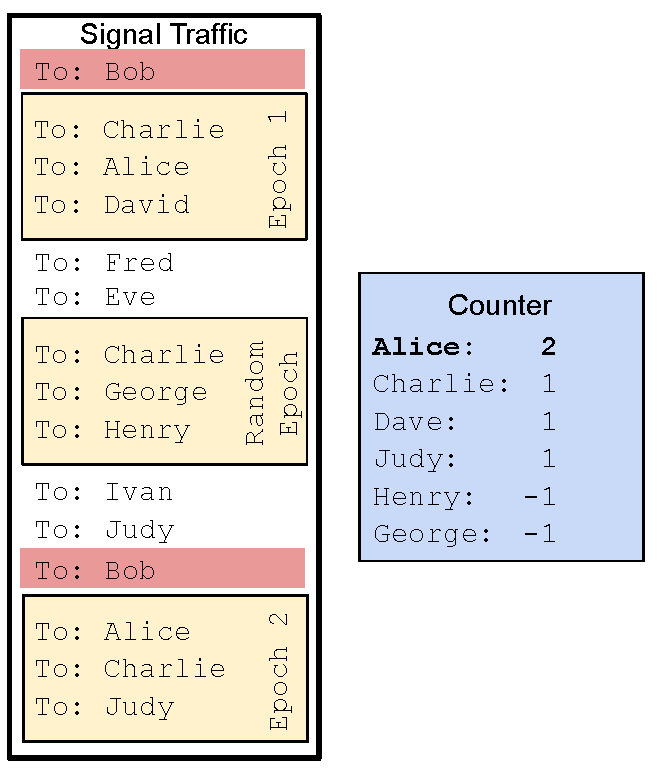
\includegraphics[clip, width=0.5\linewidth]{figs/AttackOverview.pdf}
        \caption{\textbf{Attack Overview}\,---\,% 
        Our SDA variant has the service provider (Signal) keep count of all
        users who receive messages in the \textit{epoch} after Bob receives a
        message to determine who is consistently messaging at the same time as
        Bob is receiving a message. Additionally, the service provider will
        begin an epoch at a random time to keep track of users which are
        messaging independent of the associates of Bob, and those users will be
        deducted from the counter. As such, ``popular'' users such as
        \textit{Charlie} will not mask Alice's behavior.
    }
    \label{fig:signal-AttackOverview}
\end{figure}
}

\newcommand{\LikelihoodGraph}{
\begin{figure}[t]
    \centering
    \includegraphics[width=0.9\linewidth]{figs/likelihood_receipt_response_rate.pdf}
    \caption{\textbf{Likelihood of guessing Alice is the sender}\,---\,% 
        The natural candidate for who is messaging Bob is the user who shows up
        most often in the epoch following Bob receiving a message. This graph
        analyzes the likelihood that the attacker will be correct (i.e. they will pick Alice)
        if they guess the user who has show up most often is conversing with Bob as a function
        of the number of messages Bob has received. Simulated over 1000 randomized iterations.
    }
    \label{fig:signal-AliceLikelihood}
\end{figure}
}

\newcommand{\SealedSenderStructure}{
\begin{figure}[ht]
    \centering
    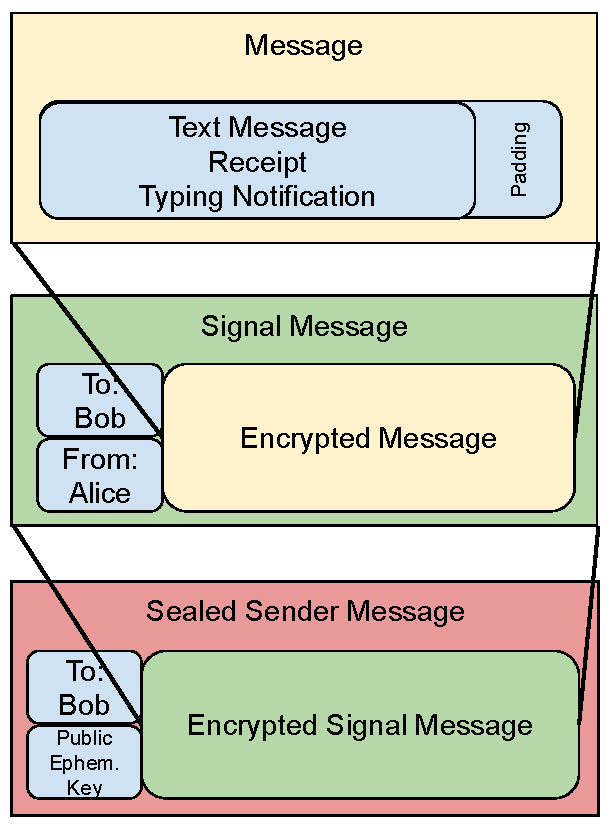
\includegraphics[width=0.5\linewidth]{figs/SealedSenderStructure.pdf}
    \caption{\textbf{Structure of Signal Messages}\,---\,% 
        All messages Alice sends to Bob through Signal (receipts, text messages,
        or events) are first padded to the next multiple of 160 bytes. The
        padded message is then encrypted under the shared key between Alice and
        Bob and then combined with `To: Bob' and `From: Alice' metadata to form
        a Signal Message. %If either Bob or Alice do not have sealed sender enabled this Signal Message will then be sent.
        If both Alice and Bob
        have sealed sender enabled then Alice will then generate an ECDHE key
        pair and derive a new shared secret with Bob's public key to encrypt
        the Signal Message and combine with `To: Bob' and the public ephemeral
        key to form a sealed sender message that will be sent to Bob.
    }
    \label{fig:signal-SealedSenderStructure}
\end{figure}
}

\newcommand{\VariantThree}{
\begin{figure}[ht]
    \centering
    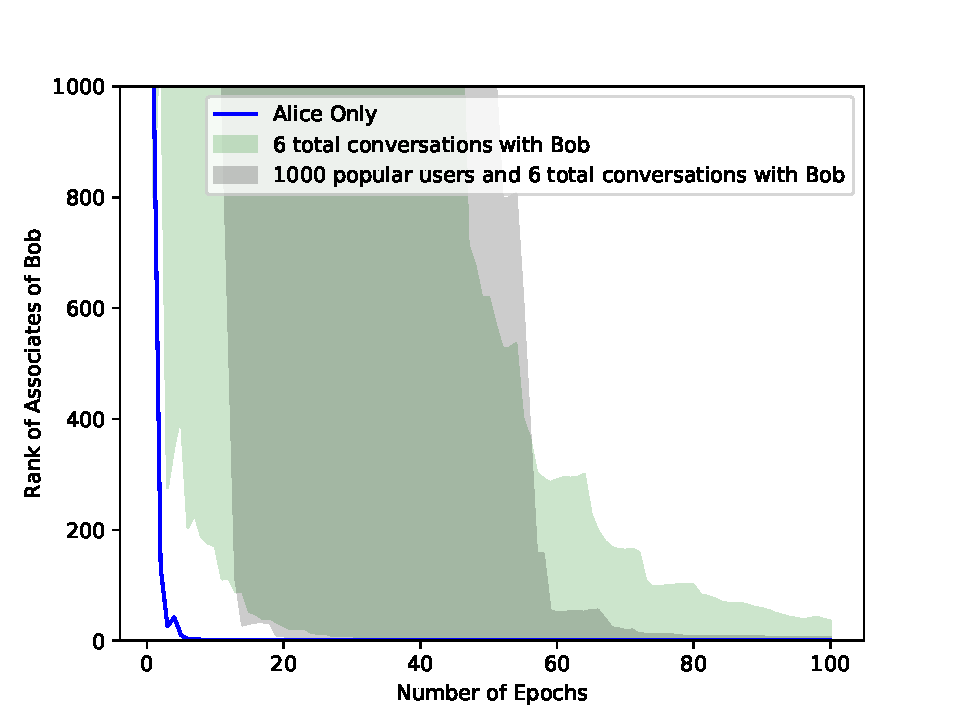
\includegraphics[width=0.9\linewidth]{figs/various_cases.pdf}
    \caption{\textbf{Effect of popular users}\,---\,% 
        We examined the effectiveness of our SDA by examining the cases where
        only Alice is messaging Bob and where Bob is being messaged by Alice and
        5 other users. The graph shows the rank of those messaging Bob, how many
        users have received more messages than those messaging Bob. When only
        Alice is messaging Bob each of the attack epochs are started by her,
        meaning her rank will very quickly drop. When multiple users are
        messaging Bob there is a range of ranks, represented by the green band
        which demonstrates the lowest ranked user messaging Bob (on the bottom)
        and the highest ranked individual messaging Bob (on the top). When
        epochs are begun by multiple users, an individual's rank takes a while
        to drop. The graph shows that for over 45 epochs one of the users
        messaging Bob has a rank of over 1000, while another user messaging Bob
        has dropped to a rank of 0 (meaning they have received a message after
        Bob received a message the most of any user in the system).
    }
    \label{fig:signal-variant3}
\end{figure}
}


\newcommand{\combinedfigures}{
\begin{figure*}[t]

    \centering
    \begin{minipage}{0.49\textwidth}
        \centering
    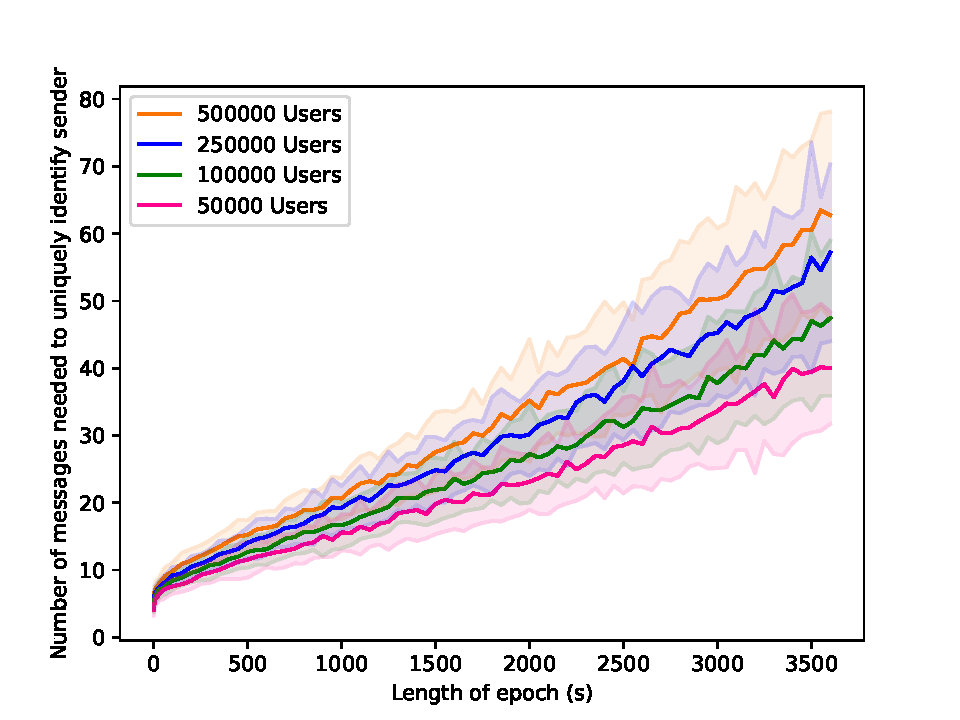
\includegraphics[width=\linewidth]{figs/epoch_effect-bars.pdf}
    \end{minipage}\hfill
    \begin{minipage}{0.49\textwidth}
        \centering
    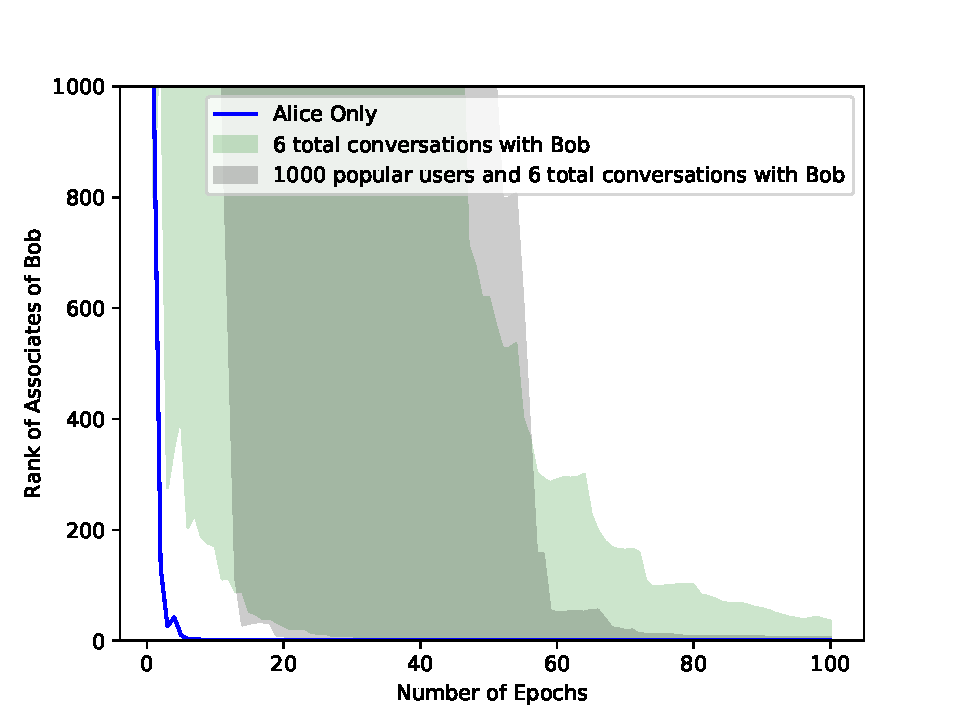
\includegraphics[width=\linewidth]{figs/various_cases.pdf}
    \end{minipage}

%     \begin{minipage}[width=0.5\linewidth]
%     \centering
%     \includegraphics[width=0.9\linewidth]{figs/epoch_effect.pdf}
%     \end{minipage}

%     \begin{minipage}[width=0.5\linewidth]
%     \centering
%     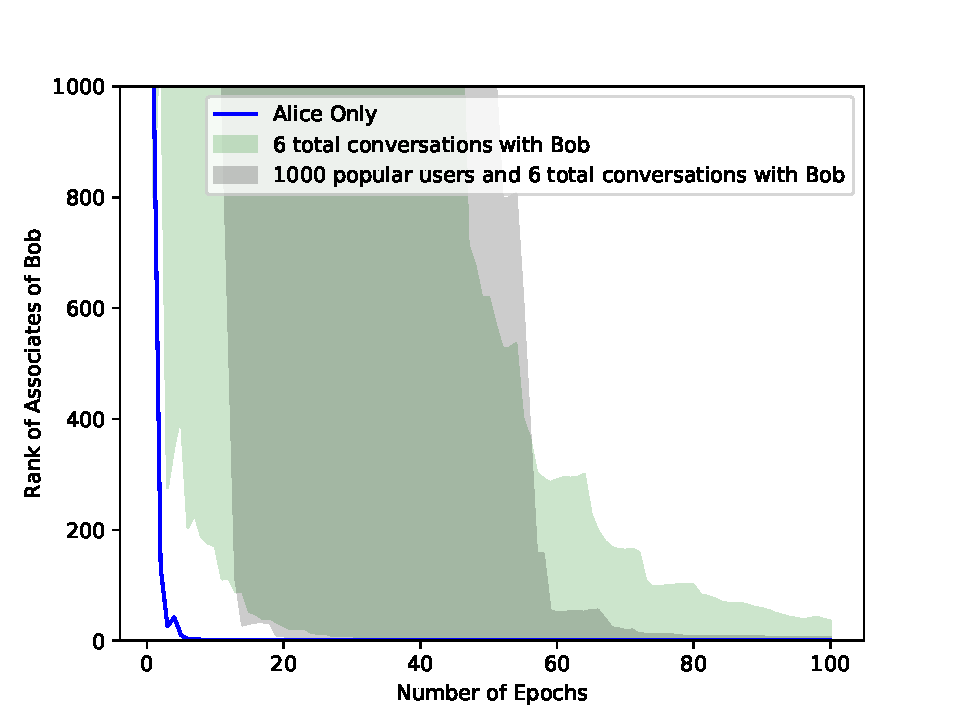
\includegraphics[width=0.9\linewidth]{figs/various_cases.pdf}
%     \end{minipage}


    \caption{\textbf{Left: Effect of delayed Read Receipts}\,---\,% 
        The attack assumes that each epoch lasts one second, and thus the log
        collects all delivery receipts that are sent within 1 second of Bob 
        receiving a sealed sender message. A possible simple solution to this
        attack is to delay delivery receipts.
        We tested the effectiveness of the attack with
        variably sized epochs and determined that if delivery receipts were
        delayed a full hour (making them effectively worthless for their
        purpose) that with a user base of 500,000 users (each sending 50
        messages a day) Bob would need to receive 60 messages from the victim
        user to identify Alice as the sender. \\
        \textbf{Right: Effect of popular users in our SDA}\,---\,% 
        We examined the effectiveness of our SDA variant by examining the cases
        where only Alice is messaging Bob and where Bob is being messaged by
        Alice and 5 other users. The graph shows the rank of those messaging
        Bob, how many users have received more messages than those messaging
        Bob. When only Alice is messaging Bob each of the attack epochs are
        started by her, meaning her rank will very quickly drop. When multiple
        users are messaging Bob there is a range of ranks, represented by the
        green band which bounds the lowest ranked user messaging Bob (on
        the bottom) and the highest ranked individual messaging Bob (on the
        top). When epochs are begun by multiple users, an individual's rank
        takes a while to drop. The graph shows that for over 45 epochs one of
        the users messaging Bob has a rank of over 1000, while another user
        messaging Bob has dropped to a rank of 0 (meaning they have received a
        message after Bob received a message the most of any user in the
        system). The black band considers the same situation, but with 1000 popular users in the system which our variant accounts for.
        }
    \label{fig:signal-combinedfigure}
\end{figure*}
}


%%% Local Variables:
%%% mode: latex
%%% TeX-master: "main"
%%% End:
